\chapter{Data Structures}
\label{ch:datastruct}

\newcommand{\lecnum}{8}
%\newcommand{\lectitle}{Data Structures}
\newcommand{\lecturer}{Frank Pfenning, Andr\'e Platzer, Rob Simmons,
  Iliano Cervesato}

\chapterTAGS{aliasing, correctness, ds-invariant, interface, pointer, safety, struct}
\maketitle

\begin{preamble}
\noindent
In this lecture we introduce the idea of \emph{imperative data structures}. So
far, the only interfaces we've used carefully are \emph{pixels} and
\emph{string bundles}. Both of these interfaces had the property that, once we
created a pixel or a string bundle, we weren't interested in changing its
contents. In this lecture, we'll talk about an interface that extends the
arrays that are primitively available in C0.

To implement this interface, we'll need to round out our discussion of types
in C0 by discussing \emph{pointers} and \emph{structs}, two tastes that
go great together. We will discuss using contracts to ensure that pointer
accesses are safe.
% , as well as the use of \emph{linked lists} to implement the
% stack and queue interfaces.  The linked list implementation of stacks and
% queues allows us to handle stacks and queues of any size.
\end{preamble}

\begin{gram}[Learning Goals]
Relating this to our learning goals, we have
\begin{description}
\item[Computational Thinking:] We illustrate the power of
  \emph{abstraction} by considering both the client-side and
  library-side of the interface to a data structure.

\item[Algorithms and Data Structures:] The abstract data structure will be one
  of our first examples of {\em abstract datatypes.}

\item[Programming:] Introduction of structs and pointers, use and
  design of interfaces.
\end{description}
\end{gram}


\section{Structs}
\label{sec:datastruct:structs}
\TAGS{safety, struct}

So far in this course, we've worked with five different C0 types ---
\lstinline'int', \lstinline'bool', \lstinline'char', \lstinline'string', and
arrays $t$\lstinline'[]' (there is a array type $t$\lstinline'[]' for every
type $t$). The character, Boolean and integer values that we manipulate, store
locally, and pass to functions are just the values themselves.  For arrays
(and strings), the things we store in assignable variables or pass to
functions are \emph{addresses}, references to the place where the data stored
in the array can be accessed.  An array allows us to store and access some
number of values of the same type (which we reference as \lstinline'A[0]',
\lstinline'A[1]', and so on).

Therefore, when entering the following commands in Coin (the outputs have been
elided),
\begin{lstlisting}[language={[coin]C}]
--> char c = '\n';
--> int i = 4;
--> string[] A = alloc_array(string, 4);
--> A[0] = "hi";
--> A[1] = "je";
--> A[2] = "ty";
--> A[3] = "lo";
\end{lstlisting}
the interpreter will store something like the following in its memory:
\begin{center}
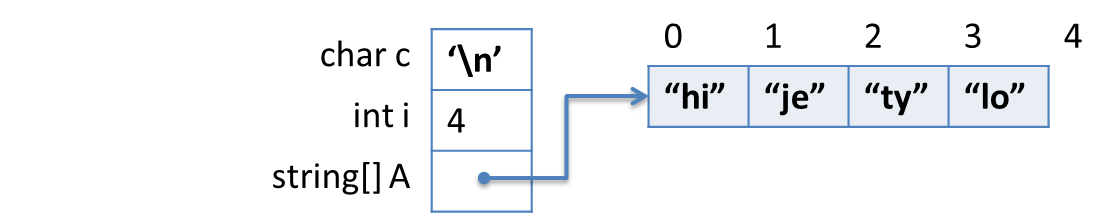
\includegraphics[width=0.85\textwidth]{img/types1.png}
\end{center}

The next data structure we will consider is the struct. A \emph{struct} can be
used to aggregate together different types of data, which helps us create
data structures.  By contrast, an array is an aggregate of elements of the
\emph{same} type.

Structs must be explicitly declared in order to define their
``shape''.  For example, if we think of an image, we want
to store an array of pixels alongside the width and height of the
image, and a struct allows us to do that:

\begin{lstlisting}[language={[C0]C}]
struct img_header {
  pixel_t[] data;
  int width;
  int height;
};
\end{lstlisting}

Here \lstinline'data',  \lstinline'width', and  \lstinline'height' are
\emph{fields} of the struct.  The declaration expresses that every image has
an array of \lstinline'pixel_t's called \lstinline'data'
as well as a \lstinline'width' and a
\lstinline'height'. This description is incomplete, as there are some missing
consistency checks --- we would expect the length of \lstinline'data' to be
equal to the \lstinline'width' times the \lstinline'height', for instance, but
we can capture such properties in a separate data structure invariant.

C0 values such as integers, characters, the address of an array are
\emph{small}. Depending on the computer, an address is either 64 bits long or
32 bits long, which means that the \emph{small types} take at most 64 bits to
represent.  Because structs can have multiple components, they can grow too
large for the computer to easily copy around, and C0 does not allow us to use
structs as locals:

\begin{lstlisting}[language={[coin]C}]
% coin structs.c0
C0 interpreter (coin) 0.3.2 'Nickel'
Type `#help' for help or `#quit' to exit.
--> struct img_header IMG;
<stdio>:1.1-1.22:error:type struct img_header not small
[Hint: cannot pass or store structs in variables directly; use
pointers]
\end{lstlisting}

Therefore, we can only create structs in allocated memory, just like
we can only store the contents of arrays in allocated memory.  (This
is true even if they happen to be small enough to fit into 32 bytes.)
Instead of \lstinline'alloc_array' we call \lstinline'alloc' which returns a
\emph{pointer} to the struct that has been allocated in memory.  Let's
look at an example in coin.
\begin{lstlisting}[language={[coin]C}]
--> struct img_header* IMG = alloc(struct img_header);
IMG is 0xFFAFFF20 (struct img_header*)
\end{lstlisting}
We can access the fields of a struct, for reading or writing,
through the notation \lstinline'p->f' where $p$ is a pointer to
a struct, and $f$ is the name of a field in that struct.
Continuing above, let's see what the default values are
in the allocated memory.
\begin{lstlisting}[language={[coin]C}]
--> IMG->data;
(default empty int[] with 0 elements)
--> IMG->width;
0 (int)
--> IMG->height;
0 (int)
\end{lstlisting}
\clearpage
We can write to the fields of a struct by using the arrow
notation on the left-hand side of an assignment.
\begin{lstlisting}[language={[coin]C}]
--> IMG->data = alloc_array(pixel_t, 2);
IMG->data is 0xFFAFC130 (int[] with 2 elements)
--> IMG->width = 1;
IMG->width is 1 (int)
--> (*IMG).height = 2;
(*(IMG)).height is 2 (int)
--> IMG->data[0] = 0xFF00FF00;
IMG->data[0] is -16711936 (int)
--> IMG->data[1] = 0xFFFF0000;
IMG->data[1] is -65536 (int)
\end{lstlisting}

The notation \lstinline'(*p).f' is a longer form of \lstinline'p->f'.  First,
\lstinline'*p' follows the pointer to arrive at the struct in memory, then
\lstinline'.f' selects the field \lstinline'f'.  We will rarely use this
dot-notation \lstinline'(*p).f' in this course, preferring the
arrow-notation \lstinline'p->f'.

An updated picture of memory, taking into account the initialization
above, looks like this:
\begin{center}
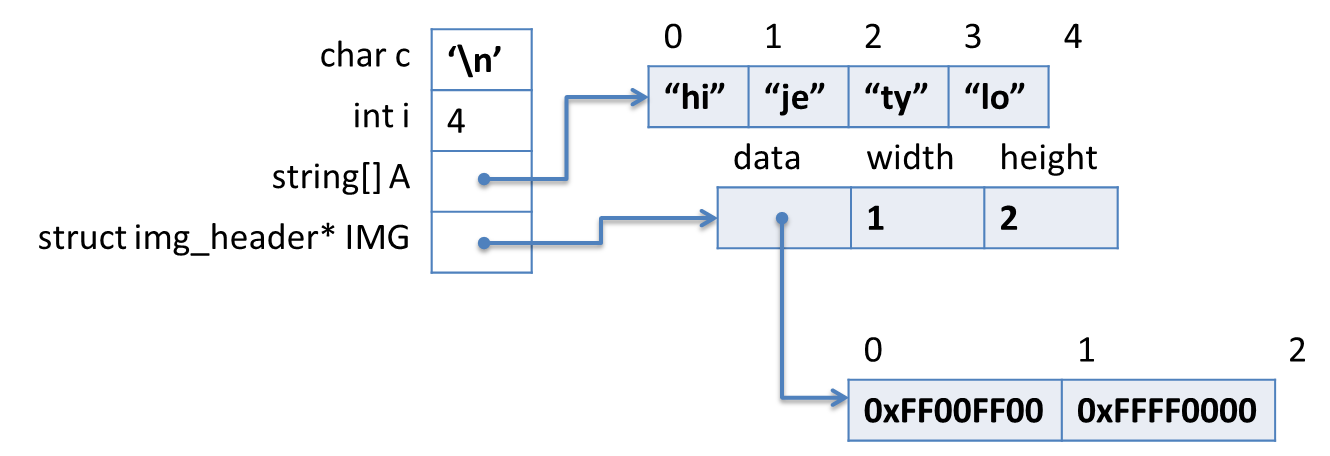
\includegraphics[width=0.85\textwidth]{img/types2.png}
\end{center}

\clearpage
\section{Pointers}
\label{sec:datastruct:pointers}
\TAGS{aliasing, pointer, safety}

As we have seen in the previous section, a pointer is needed to refer
to a struct that has been created in allocated memory.  In can also be
used more generally to refer to an element of arbitrary type that has
been created in allocated memory.  For example:
\begin{lstlisting}[language={[coin]C}]
--> int* ptr1 = alloc(int);
ptr1 is 0xFFAFC120 (int*)
--> *ptr1 = 16;
*(ptr1) is 16 (int)
--> *ptr1;
16 (int)
\end{lstlisting}
In this case, we refer to the value of \lstinline'p' using the notation
\lstinline'*p', either to read (when we use it inside an expression) or to
write (if we use it on the left-hand side of an assignment).

So we would be tempted to say that a pointer value is simply
an address.  But this story, which was correct for arrays,
is not quite correct for pointers. There is also a special
value \lstinline'NULL'.  Its main feature is that \lstinline'NULL' is
not a valid address, so we cannot dereference it to obtain
stored data.  For example:
\begin{lstlisting}[language={[coin]C}]
--> int* ptr2 = NULL;
ptr2 is NULL (int*)
--> *ptr2;
Error: null pointer was accessed
Last position: <stdio>:1.1-1.3
\end{lstlisting}
Graphically, \lstinline'NULL' is sometimes represented with the ground
symbol, so we can represent our updated setting like this:
\begin{center}
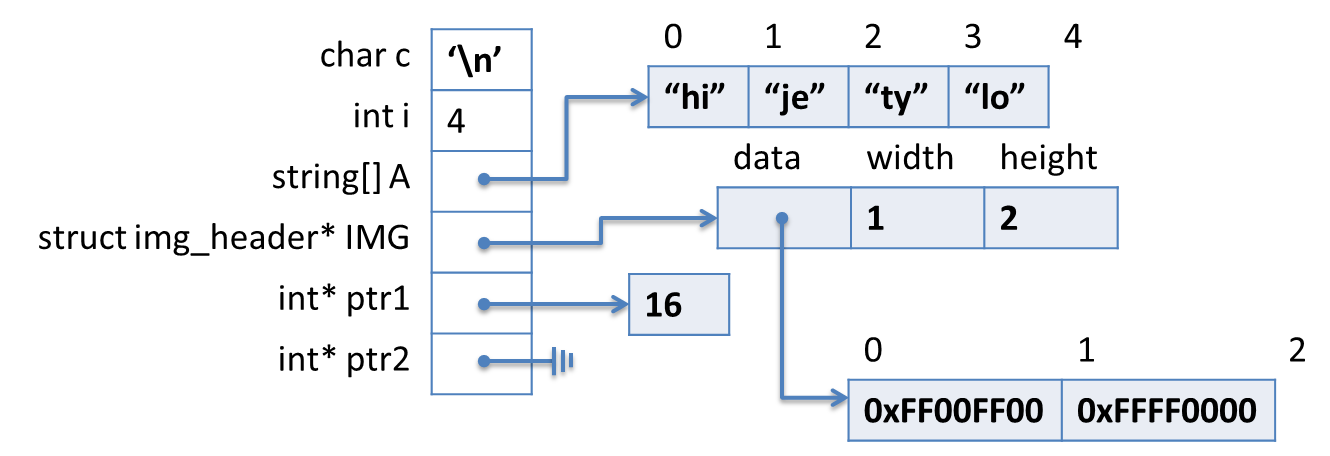
\includegraphics[width=0.85\textwidth]{img/types3.png}
\end{center}

To rephrase, we say that a pointer value is an address, of which there
are two kinds.  A valid address is one that has been allocated
explicitly with \lstinline'alloc', while \lstinline'NULL' is an invalid address.
In C, there are opportunities to create many other invalid addresses,
as we will discuss in another lecture.

Attempting to dereference the null pointer is a safety violation in
the same class as trying to access an array with an out-of-bounds
index.  In C0, you will reliably get an error message, but in C the
result is undefined and will not necessarily lead to an error.
Therefore:
\begin{quote}\it
  Whenever you dereference a pointer $p$, either as \lstinline'*p'
  or \lstinline'p->f', you must have a reason to know that $p$
  cannot be \lstinline'NULL'.
\end{quote}
In many cases this may require function preconditions or loop
invariants, just as for array accesses.

%%% TODO IT WOULD BE GOOD TO TALK ABOUT LVALUES HERE


\section{Creating an interface}
\label{sec:datastruct:interface}
\TAGS{interface}

The next ten lectures for this class will focus on building, analyzing, and
using different data structures. When we're thinking about implementing data
structures, we will almost always use pointers to structs as the core of our
implementation.

In the rest of this lecture, we will build a data structure for
\emph{self-sorting arrays}.  Like arrays, they will contain a fixed
number of elements of a given type that can be accessed through an
index (we will limit ourselves to self-sorting arrays of strings).
Unlike C0 arrays, the values in a self-sorting array are sorted, and
remain so as we update its values.  That allows a programmer using our
self-sorting arrays to look for elements using binary search, in
$O(\log{n})$ time if $n$ is the number of contained elements.

Self-sorting arrays work mostly like arrays of strings.  The primitive
operations that C0 provides on string arrays are the ability to create
a new array, to get a particular index of an array, and to set a
particular index in an array.  We capture these as three functions
that act on an abstract type \lstinline'ssa_t' (mnemonic for
\underline{s}elf-\underline{s}orting \underline{a}rray
\underline{t}ype):
\begin{lstlisting}[language={[C0]C}]
// typedef _______ ssa_t;
ssa_t  ssa_new(int size);        // ~ alloc_array(string, size)
string ssa_get(ssa_t A, int i);            // ~ A[i]
void   ssa_set(ssa_t A, int i, string x);  // ~ A[i] = x
\end{lstlisting}
But this is not a complete picture! An interface needs to also capture
the preconditions necessary for using that abstract type
\emph{safely}. For instance, we know that safety of array access
requires that we only create non-negative-length arrays and we never
try to access a negative element of an array:
\begin{lstlisting}[language={[C0]C}]
ssa_t  ssa_new(int size)       /*@requires size >= 0 @*/;
string ssa_get(ssa_t A, int i) /*@requires 0 <= i;   @*/;
\end{lstlisting}
This still isn't enough: our contracts need to ensure an upper bound
so that we don't access the element at index 100 of a length-12
array. We don't have the \length{()} method, as it is a primitive for
C0 arrays, not our new \lstinline'ssa_t' type. So we need an
additional function in our interface to get the length, and we'll use
that in our contracts.
\begin{lstlisting}[language={[C0]C}]
int ssa_len(ssa_t A);
string ssa_get(ssa_t A, int i)
  /*@requires 0 <= i && i < ssa_len(A); @*/ ;
\end{lstlisting}
It's important to emphasize what just happened. Because we want the
type \lstinline'ssa_t' to be \emph{abstract}, we can't use \length{}
in a contract: we can only use \length{} for arrays. Because we have
to be able to write a contract that explains how to use the data type
safely, we need to extend our interface with a new function
\lstinline'ssa_len'. But because this function is in the interface,
the client can access the length of the array --- something that can't
be done for C0 arrays (outside of a contract)! So we \emph{do} know
something about \lstinline'ssa_t' now: it can't just be
\lstinline'string[]', because if it was there would be no way to
implement \lstinline'ssa_len'.

For this reason, we're going to say that \lstinline'ssa_t' is not an
unknown type but that it is an unknown \emph{pointer} type. The
updated pseudo-typedef below shows how we indicate this:

\begin{lstlisting}[language={[C0]C}]
// typedef ______* ssa_t;

int ssa_len(ssa_t A)
  /*@requires A != NULL; @*/;

ssa_t ssa_new(int size)
  /*@requires 0 <= size; @*/
  /*@ensures \result != NULL; @*/
  /*@ensures ssa_len(\result) == size; @*/;

string ssa_get(ssa_t A, int i)
  /*@requires A != NULL; @*/
  /*@requires 0 <= i && i < ssa_len(A); @*/;

void ssa_set(ssa_t A, int i, string x)
  /*@requires A != NULL; @*/
  /*@requires 0 <= i && i < ssa_len(A); @*/;
\end{lstlisting}
Admitting that \lstinline'ssa_t' is a pointer also means that we
have to add a lot of \lstinline'NULL' checks to the interface --- as
the client of the \lstinline'ssa_t' type, we know that a value of
this type is either a valid pointer to the self-sorting array data
structure, or it is \lstinline'NULL'.


\section{The Library Perspective}
\label{sec:datastruct:library}
\TAGS{correctness, safety}

When we implement the library for \lstinline'ssa_t', we will declare
a type \lstinline'ssa' as a synonym for %
\lstinline'struct ssa_header', which has a \lstinline'length' field
to hold the length and a \lstinline'data' field to hold the actual
array.
\begin{lstlisting}[language={[C0]C}]
struct ssa_header {              // Implementation type
  int length;
  string[] data;
};
typedef struct ssa_header ssa;   // Abbreviation

typedef ssa* ssa_t;              // Interface type
\end{lstlisting}
The last line is where we make a connection between the interface
type \lstinline'ssa_t' exported to the user by the interface, and
the type \lstinline'ssa' (or equivalently %
\lstinline'struct ssa_header') %
the library uses to implement the exported functionalities.  As
promised, it is a pointer type.  We usually write it as the very last
line of the implementation.

Inside the library implementation, we'll use \lstinline'ssa*' instead of
\lstinline'ssa_t' to emphasize that we're manipulating a pointer structure.
Outside, we use exclusively \lstinline'ssa_t' as our abstract type of supped
up arrays.  Using this knowledge, we can begin to implement the array
interface from the library side, though we immediately run into safety issues.
\begin{lstlisting}[language={[C0]C}]
int ssa_len(ssa* A)
//@requires A != NULL;
{
  return A->length;
}

string ssa_get(ssa* A, int i)
//@requires A != NULL;
//@requires 0 <= i && i < ssa_len(A);
{
  return A->data[i];
}
\end{lstlisting}
In both cases, the precondition \lstinline'A != NULL' allows us to say
that the dereferences \lstinline'A->length' and \lstinline'A->data' are
safe. But how do we know \lstinline'A->data[i]' is not an
out-of-bounds array access?  We don't --- the second precondition of
\lstinline'ssa_get' just tells us that \lstinline'i' is nonnegative
and less than whatever \lstinline'ssa_len' returns!

If we want to use the knowledge that \lstinline'ssa_len(A)' returns
the length of \lstinline'A->data', then we'd need to add
\result\lstinline' == '\length{(A->data)} as a postcondition of
\lstinline'ssa_len'\ldots

\ldots and we can only prove that postcondition true if we add the
precondition \lstinline'A->length == '\length{(A->data)} to
\lstinline'ssa_len'\ldots

\ldots and if we do that, it changes the safety requirements for the
call to \lstinline'ssa_len' in the preconditions of
\lstinline'ssa_get', so we also have to add the precondition\linebreak[4]
\lstinline'A->length == '\length{(A->data)} to \lstinline'ssa_get'.

The user, remember, didn't need to know anything about this, because
they were ignorant of the internal implementation details of the
\lstinline'ssa_t' type.  As long as the user respects the interface,
only creating \lstinline'ssa_t''s with \lstinline'ssa_new' and only
manipulating them with \lstinline'ssa_len', \lstinline'ssa_get',
and \lstinline'ssa_set', they should be able to expect that the
contracts on the interface are sufficient to ensure safety. But we
don't have this luxury from the library perspective: all the functions
in the library's implementation are going to depend on all the parts
of the data structure making sense with respect to all the other
parts. We'll capture this notion in a new kind of invariant, a
\emph{data structure invariant}.


\section{Data Structure Invariants}
\label{sec:datastruct:ds-invariant}
\TAGS{correctness, ds-invariant, safety}

We can apply operational reasoning as library designers to say that,
as long as the \lstinline'length' field of an \lstinline'ssa' is set
correctly by \lstinline'ssa_new', it must remain correct throughout
all calls to \lstinline'ssa_get' and \lstinline'ssa_set'. But, as with
operational reasoning about loops, this is an error-prone way of
thinking about our data structures. Our solution in this case will be
to capture what we know about the well-formedness of an array in an
invariant; we expect that any \lstinline'ssa' being handled by the
user will satisfy this data structure invariant.

The above invariants for self-sorting arrays are pretty simple: a
\lstinline'ssa' is well-formed if it is a non-\lstinline'NULL'
pointer to a struct where \length{(A->data)} %
\lstinline' == A->length'.  %
They capture safety but do not say anything about the array being
sorted.  We will add a correctness invariant, that the array be in
fact sorted.  This is achieved through a function
\lstinline'is_sorted' which is implemented similarly to the
corresponding function for arrays of integers --- it can be found in
the code accompanying this lecture.  If we try to turn this into a
mathematical statement that captures the overall well-formedness
requirements for our implementation, we get the \emph{specification
  function} \lstinline'is_ssa':
\begin{lstlisting}[language={[C0]C}]
bool is_ssa(ssa* A) {
  return A != NULL
      && is_sorted(A)
      && is_array_expected_length(A->data, A->length);
}
\end{lstlisting}
While we would like \lstinline'is_array_expected_length' to be a function
that returns \lstinline'true' when the given array has the expected length
and \lstinline'false' otherwise, the restriction of length-checking to
contracts makes this impossible to write in C0. In this one case, we'll
allow ourselves to write a data structure invariant that might raise
an assertion error instead of returning \lstinline'false':
\begin{lstlisting}[language={[C0]C}]
bool is_array_expected_length(string[] A, int length) {
  //@assert \length(A) == length;
  return true;
}
\end{lstlisting}
Whenever possible, however, we prefer data structure invariants that
return \lstinline'true' or \lstinline'false' to data structures that raise
assertion failures.

The data structure invariant, then, implies the postcondition of
\lstinline'ssa_len', and so the function \lstinline'ssa_get' will require the
data structure invariant to hold as well, satisfying the precondition
of \lstinline'ssa_len'.
\begin{lstlisting}[language={[C0]C}]
int ssa_len(ssa* A)
//@requires is_ssa(A);
//@ensures \result == \length(A->data);
{
  return A->length;
}

string ssa_get(ssa* A, int i)
//@requires is_ssa(A);
//@requires 0 <= i && i < ssa_len(A);
{
  return A->data[i];
}
\end{lstlisting}

\clearpage
Functions that create new instances of the data structure should
ensure that the data structure invariants hold of their results, and
functions that modify data structures should have postconditions to
ensure that none of those data structure invariants have been
violated.
\begin{lstlisting}[language={[C0]C}]
ssa* ssa_new(int size)
//@requires 0 <= size;
//@ensures is_ssa(\result);
{
  struct ssa_header* A = alloc(struct ssa_header);
  A->length = size;
  A->data = alloc_array(string, size);
  return A;
}

void ssa_set(ssa* A, int i, string x)
//@requires is_ssa(A);
//@requires 0 <= i && i < ssa_len(A);
//@ensures is_ssa(A);
{
  A->data[i] = x;

  // Move x up the array if needed
  for (int j=i; j < A->length-1 &&
                string_compare(A->data[j],A->data[j+1]) > 0;
       j++)
    //@loop_invariant i <= j && j <= A->length - 1;
    swap(A->data, j, j+1);

// Move x down the array if needed
  for (int j=i; j > 0 &&
                string_compare(A->data[j],A->data[j-1]) < 0;
       j--)
    //@loop_invariant 0 <= j && j <= i;
    swap(A->data, j, j-1);
}
\end{lstlisting}
The code below \lstinline'A->data[i] = x' moves \lstinline'x' up or
down the array \lstinline'A->data' to ensure that the sortedness
invariant remains satisfied once the function returns.  As a
consequence, it is unlikely that a subsequent call to
\lstinline'ssa_get(A, i)' will return \lstinline'x' as its value.
This differs from C0 arrays, for which elements can always be found
where we just put them.

Now that we have added data structure invariants, our operational
reasoning for why \lstinline'ssa_get' was safe can be formalized as
an invariant. Any client that respects the interface will only ever
get and will only ever manipulate arrays that satisfy the data
structure invariants, so we know that the data structure invariants
we're counting on for safety will hold at runtime.


\section{Invariants Aren't Usually Part of the Interface}
\label{sec:datastruct:invariant-interface}
\TAGS{ds-invariant, interface}

When we have interfaces that hide implementations from the user, then
the data structure invariant, captured here by the function
\lstinline'is_ssa', should \emph{not} be a part of the
interface. Clients don't need to know that the internal invariants are
satisfied; as long as they're using \lstinline'ssa' according to the
interface, their invariants should be satisfied.

This applies to all aspects of \lstinline'is_ssa', in particular to
the correctness invariant checked by the function
\lstinline'is_sorted'.  But how shall the client be sure that the
elements of a self-sorting array are and remains sorted as it is used?
The client may trust the developer of the data structure library.
Another option is to write a client-side version of
\lstinline'is_sorted' using \emph{only the operations exported by the
  interface}.
